
%%% Local Variables:
%%% mode: latex
%%% TeX-master: t
%%% End:

\documentclass{standalone}
\usepackage{tikz}
\usepackage{amsmath}
\usepackage{pgfplots}
\usetikzlibrary{matrix,arrows,calc,fadings,decorations.pathreplacing,positioning}
\begin{document}
\pagestyle{empty}

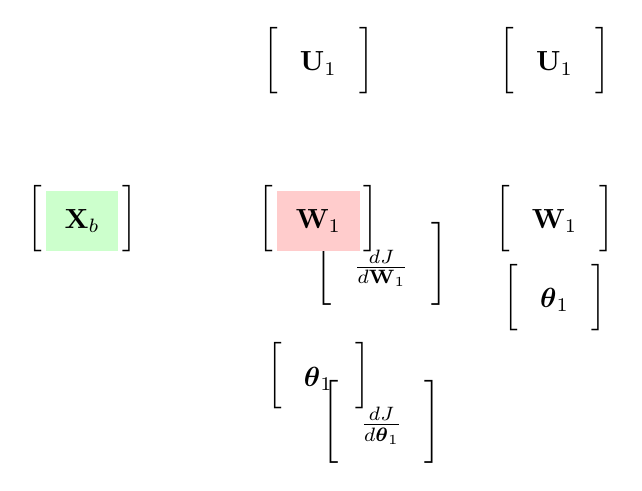
\begin{tikzpicture}[shorten >=1pt,->,draw=black!50, node distance=\layersep]

\matrix[fill=green!20, matrix of math nodes, left delimiter = [, right delimiter = {]}] (Xb)
 at (0,0)  {\mathbf{X}_b\\};

\matrix[matrix of math nodes, left delimiter = [, right delimiter = {]}] (Xb)
 at (3,2)  {\mathbf{U}_1\\};
\matrix[matrix of math nodes, left delimiter = [, right delimiter = {]}] (Xb)
 at (3.8,-0.6)  {\frac{dJ}{d\mathbf{W}_1}\\};
\matrix[fill=red!20, matrix of math nodes,
 left delimiter = [, right delimiter = {]}] (Xb)
 at (3,0)  {\mathbf{W}_1\\};
\matrix[matrix of math nodes, left delimiter = [, right delimiter = {]}] (Xb)
 at (3.8,-2.6)  {\frac{dJ}{d\boldsymbol{\theta}_1}\\};
\matrix[matrix of math nodes, left delimiter = [, right delimiter = {]}] (Xb)
 at (3,-2)  {\boldsymbol{\theta}_1\\};

\matrix[matrix of math nodes, left delimiter = [, right delimiter = {]}] (Xb)
 at (6,2)  {\mathbf{U}_1\\};
\matrix[matrix of math nodes, left delimiter = [, right delimiter = {]}] (Xb)
 at (6,0)  {\mathbf{W}_1\\};
\matrix[matrix of math nodes, left delimiter = [, right delimiter = {]}] (Xb)
 at (6,-1)  {\boldsymbol{\theta}_1\\};
\end{tikzpicture}
% End of code
\end{document}